\documentclass[article, onecolumn, 12pt]{IEEEtran}
\IEEEoverridecommandlockouts
% The preceding line is only needed to identify funding in the first footnote. If that is unneeded, please comment it out.
\usepackage{cite}
\usepackage{amsmath,amssymb,amsfonts}
\usepackage{algorithmic}
\usepackage{graphicx}
\usepackage{textcomp}
\usepackage{xcolor}
\usepackage{hyperref}
\usepackage{float}
\def\BibTeX{{\rm B\kern-.05em{\sc i\kern-.025em b}\kern-.08em
    T\kern-.1667em\lower.7ex\hbox{E}\kern-.125emX}}
\begin{document}

\title{Utilizing Model Checking to Support Constructive Proofs\\
of the MyCHIPs Distributed Digital Currency Protocol}

\author{\IEEEauthorblockN{Kyle Storey}
\IEEEauthorblockA{\textit{Brigham Young University} \\
Provo, Utah \\
kyle.r.storey@gmail.com}
}

\maketitle

\begin{abstract}
This work will explore how combining model checking and constructive proofs can be an effective method for formally verifying complex distributed protocols. MyCHIPs, a novel digital currency based on the value of personal credit\cite{bateman_myCHIPs}, has been selected as a case study because it requires certain properties to hold on a non-trivial distributed algorithm. 
This work will use model-checking to examine every possible state of a system with a small number of agents and verify that certain properties hold. By defining the partial order of events that is imposed by an algorithm, the set of all traces of events that are possible in a given system can be defined by construction. Using this constructively defined set of traces, this work will produce mechanized proofs that a system with a new agent added conforms to the the original system in that the observable behavior of the agents in the original model is unchanged. We can use this as an inductive step to prove that the properties verified in the small example extends to a system with any number of agents. 

\end{abstract}

\section{Introduction}
Proof assistants are very effective at verifying properties in inductively defined systems. This allows proof assistants to reason about systems with an unbounded number of agents. However, proof assistants are not well equipped to verify temporal properties.
Model checking is very effective at verifying temporal properties of distributed systems, but model checking can be computationally complex and it is only practical when applied to simple models with a small number of agents. This work will leverage model checking to verify temporal properties in a small system. It will then utilize proof assistants to extend these model checking results and prove that the properties continue to hold for a system with an unbounded number of agents. 

The intuition in the proof is to show that adding an additional agent to the system will not change the behavior of any of the agents already in the system. If the behavior of the agents in the original system is unchanged the verified properties will still hold in the system with an additional agent.
This is done by defining a partial order that is imposed by the system's protocol, and using that partial order to define the set of all possible traces of events that can occur in the protocol for a small number of agents. This is the same set of traces that the model checker previously verified. This forms the base case in an inductively defined system. We then add a new agent into the system and define the set of all possible traces in this new larger system. If the set of traces produced by the system with N+1 agents is projected to only include events that affect agents in the system with N agents, and the resulting set of traces is equivalent to the set of traces in the system with N agents, it follows that the properties in the system with N agents continue to hold in the system with N+1 agents. This process is often referred to as \emph{conformance}. 

This whole process is demonstrated in a case study of MyCHIPs. MyCHIPs employs a distributed protocol as a means of facilitating the trade of goods and services between trusting partners. There are many temporal properties that must hold for MyCHIPs to meet its security and functionality requirements. This work will verify several of those properties.

\section{Driving Example}

MyCHIPs is a novel digital currency based on a distributed network of trusting trading partners. CHIPs in the MyCHIPs network, are units of value that are backed by a promise that the issuer will provide some good or service to the receiver at some future time. In this way CHIPs can be thought of as an IOU. To prevent abuse, CHIPs in the MyCHIPs network are designed to be non-transferable. This complicates transactions because non-transferable tokens are not fungible. To overcome this, MyCHIPs implements a method to make CHIPs \emph{virtually fungible} using a distributed algorithm called a \emph{credit lift}. \cite{bateman_myCHIPs}

A lift makes CHIPs virtually fungible by identifying a circuit where every entity holds CHIPs issued by their predecessor in the circuit. The lift algorithm arranges for each entity in the cycle to forgive the debt of their predecessor to get the same amount forgiven by their successor. 
 
\begin{figure}[H]
    \centering
    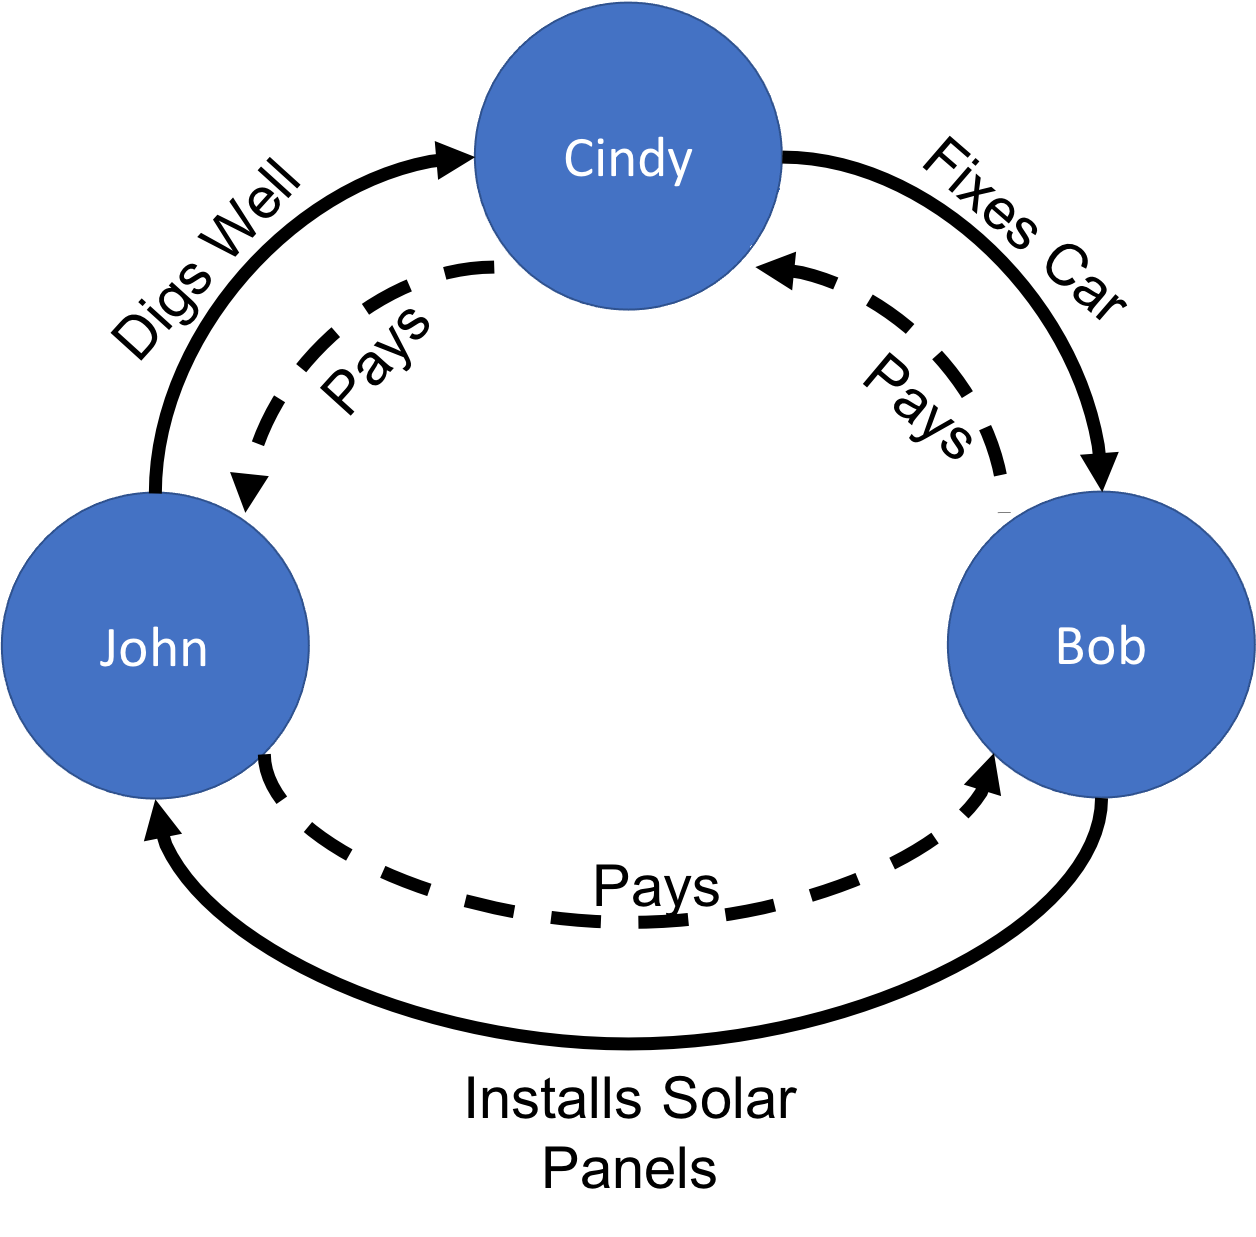
\includegraphics[scale=0.3]{ExampleCircuit.png}
    \caption{Example Circuit}
    \label{fig:liftProt}
\end{figure}
How this facilitates trade can be better understood by considering a barter system that involves more than two parties. 
For example, Bob needs his car fixed, John wants solar panels installed on his roof, and Cindy wants a well dug. Cindy knows how to fix cars, Bob knows how to install solar panels, and John is able to dig a well. See Fig. \ref{fig:liftProt} for a graphical representation of this arrangement. If they get together, they can work out a trade where John digs the well for Cindy, Cindy fixes Bob's Car, and Bob installs John's solar panels. Everyone would be happy.

But it is difficult to identify the these cycles before every transaction. This is where money comes in. Using government-backed money like dollars or euros, Bob might get a loan from a bank so he could pay Cindy to fix his car. Cindy would then give that money to John to dig the well, and John would give the money back to Bob to install the solar panels. Bob then has the money to repay his loan (but he may need to pay a little interest). MyCHIPs solves the same problem but instead does so by explicitly finding these cycles of value. Each person providing goods or services accepts CHIPs as an IOU for the exchange. Then a successful lift discovers this cycle of value and clears the debts of all involved.

If John, Bob, and Cindy were to perform a credit lift by hand, Bob would ask Cindy to fix his car and he might agree to give Cindy 10 CHIPs for her work. Likewise, John gives Bob 10 CHIPs and Cindy gives John 10 CHIPs. They each keep a \emph{tally} that records how many CHIPs each person has given each other. One day, Cindy is talking with Bob and learns that John gave Bob 10 CHIPs. She realizes that because Bob gave her 10 CHIPs, and she gave John 10 CHIPs there is a cycle and she can initiate a lift. Cindy \emph{promises} Bob that she will forgive his debt (by giving him 10 CHIPs back to neutralize his CHIPs) if he can get John to do the same for her. By doing this, she takes on the role of the \emph{originator} of the lift. They part ways, and the next time Bob sees John, Bob gives John a similar promise. When John sees Cindy, he gives her a similar promise and Cindy knows the deal is on. Cindy \emph{commits} and she signs a note saying she will forgive Bob's debt and gives it to John. John gives Cindy 10 CHIPs and their tally now totals to 0. When John sees Bob, he gives him Cindy's note and Bob gives John 10 CHIPs as he promised. Then Bob gives Cindy her note back and she gives him 10 CHIPs as promised. We can see this exchange allows for virtual fungibility: each person trades some CHIPs they have received to get back some CHIPs they have given out. 
This resets their balances so they can then give more CHIPs out again in exchange for future goods they will need. 

A lift in the MyCHIPs protocol works similarly but adds a few details to cover edge cases and allow the process to be done remotely and digitally.
As in our example with John, Cindy and Bob, the debt clearing is done in two steps. First, each entity \emph{promises} to send CHIPs to their predecessor to neutralize some of the CHIPs they have received. Then, once all have promised, the lift \emph{commits} and each node sends CHIPs as promised. They keep track of these transactions of CHIPs using a \emph{tally}. Once all have sent CHIPs, each entity's \emph{balance}--the difference between the number of CHIPs they have sent and the number of CHIPs they have received--remains the same, but they have cleared their liabilities. Unfortunately, sometimes entities on the MyCHIPs network may lose connectivity or otherwise become \emph{inactive}. An inactive node may not send or receive messages for an unbounded amount of time. It is not acceptable for lifts to hang in an unfinished state indefinitely. To prevent this, each lift is given a time limit, represented by a timestamp at which time the lift can no longer be committed. Because we don't expect entities on the network to have synchronized clocks, a referee is appointed whose clock is considered authoritative and acts as a consensus object. If the originator requests to commit before the timeout, the referee provides a digital signature that is proof that the lift has been committed. If the lift is not committed before the timeout, the lift becomes \emph{nullified} and the referee will never provide a signature for that lift.

MyCHIPS claims certain properties hold for its lift protocol but makes no formal arguments to prove those claims. The work proposed in this thesis is to formally prove some of those properties. These properties must hold for all compliant nodes on the network and must hold regardless of the number of nodes that participate in a lift. 

The properties this work will verify are as follows:

\begin{enumerate}
\item Lifts always eventually are committed or nullified for every active node. 
\item At the final state of the lift, every active node agrees that the lift was committed or every active node agrees the lift was nullified. 
\item The balance of every active node on the final state of the lift is equal to or greater than its initial balance.
\item Every active pair of nodes on the final state of the lift agree on their shared tally.
\end{enumerate}

In this work, we will prove these properties hold in a system with just an originator, a referee, and one relay--a node that is not an originator or a referee-- using a model checker. We will define a partial order of events based on the constraints of the protocol. Then in the proof assistant Coq, we will define the set of traces of events that are allowed by the partial order. This enumerates the same set of traces checked by our model checker. We will use this set of traces as an expression context as described by Dill \cite{dill_trace_theory} to define a conformation relation. This conformation relation will determine if one subsystem can be substituted for another subsystem and the remainder of the system's behavior will not change.
Using the model checking results as a base case, we will prove that the set of traces produced by a chain of n+1 relay nodes conforms to the set of traced produced by n relay nodes and inductively argue that the properties verified by model checking still hold for any number of nodes.


\section{Thesis}
Model-checking can prove the properties hold for a three-node system running the lift protocol. The model checking results can be generalized to any number of nodes in the protocol with Coq by abstracting the system to three roles: originator, referee, and relay where there can be any number of relays and proving that a chain of $n+1$ relay nodes will behave equivalently to a chain of $n$ relay nodes.

\section{Lift Protocol}
This section formalizes the MyCHIPs protocol as described the introduction. The protocol consists of three phases: discovery, promise, and commit. In the discovery phase, a circuit is identified where each entity is willing to participate in a lift. The correctness of the discovery phase is not critical because no transfer of value occurs during this phase. As such, this phase will not be verified.
Fig. \ref{fig:liftSequence} describes an example of a sequence of messages that would be passed in a typical lift during the promise and commit phases.

The originator initiates the lift by sending Relay 1 a lift record. This record has the lift value, the network ID of a referee that the originator selects, and a timeout timestamp. Sending this lift record represents a promise and once Relay 1 obtains the referee's signature they can immediately add the number of chips specified in the lift record to it's tally with the originator.

\begin{figure}
    \centering
    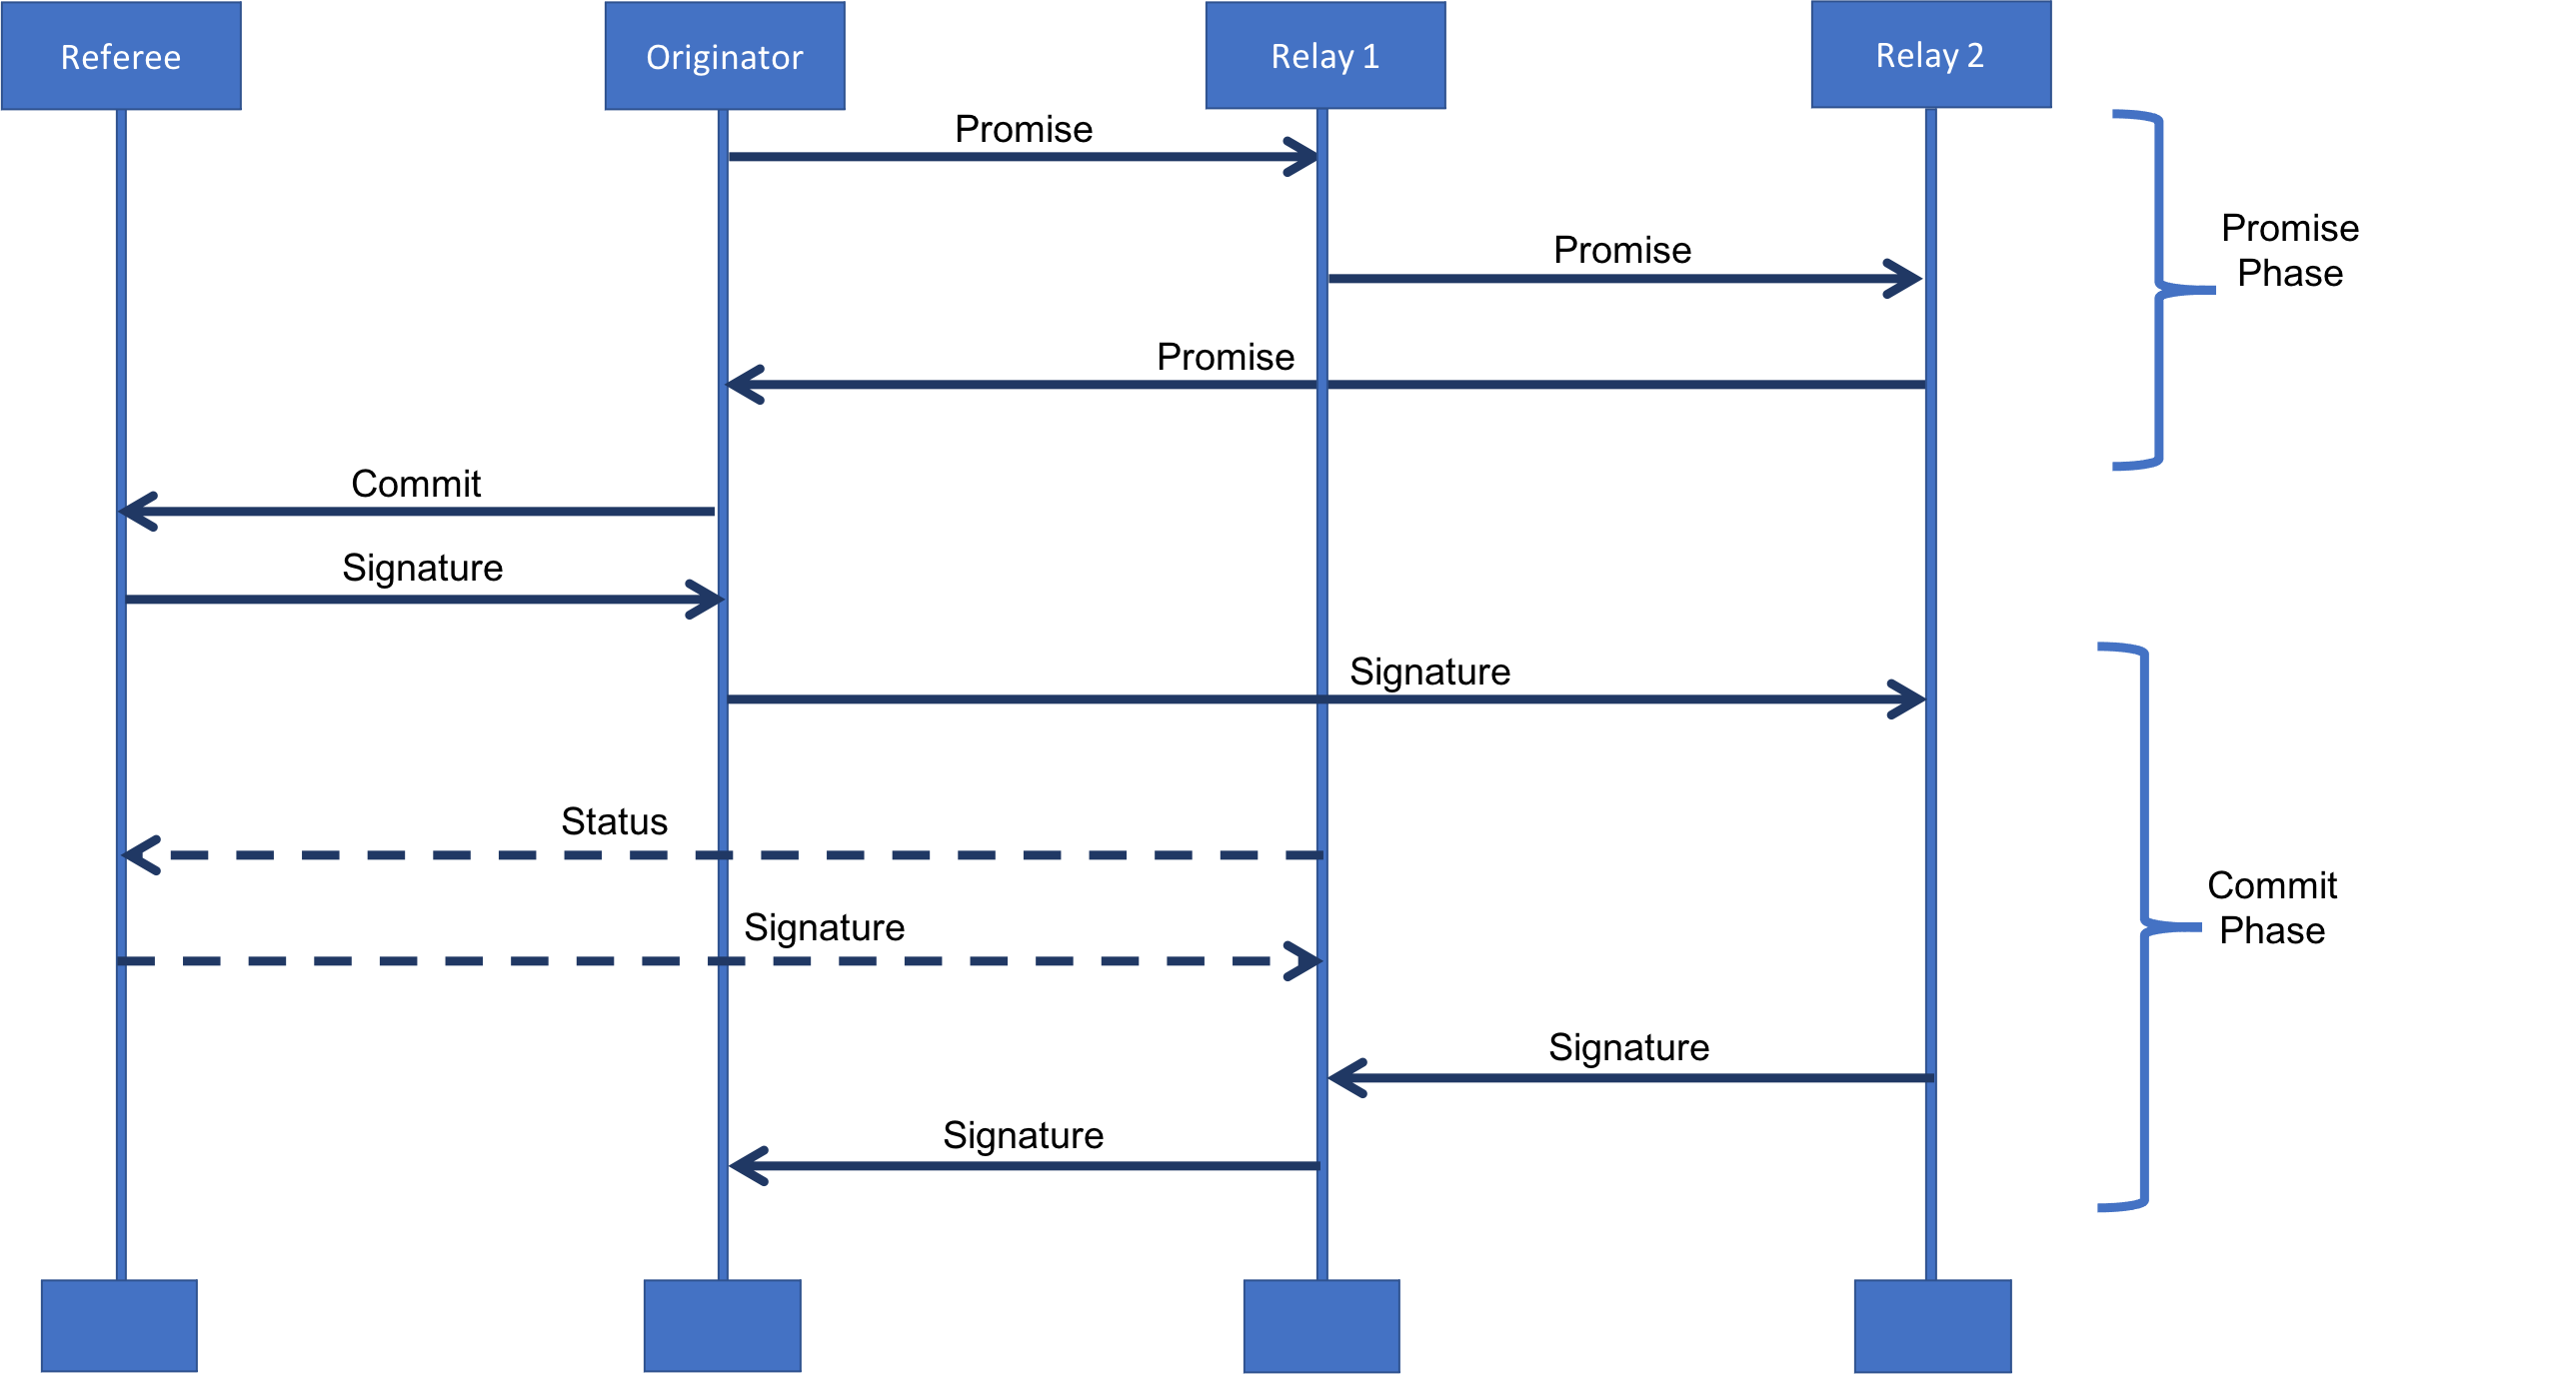
\includegraphics[scale=0.45]{SequenceDiagramLifeline.png}
    \caption{Lift Protocol Sequence Example}
    \label{fig:liftSequence}
\end{figure}

When Relay 1 receives the lift record, it first confirms that it trusts the referee to be fair and available, and it confirms that the timeout timestamp is acceptable. If the referee is not trusted, or the known route to the target is no longer valid (for instance if it was used in a different lift and the node no longer has debt on that route to clear) it may choose to not continue. The node can optionally return a message indicating that it does not intend to complete the lift, or the node can simply ignore the message and wait for the lift to timeout. In our model, nodes ignore messages if they do not intend to participate in a lift. In our example, Relay 1 wishes to participate, so it forwards the lift record along with its own promise to Relay 2. Relay 2 then similarly evaluates the lift and decides to forward a promise to its predecessor which happens to be the originator. 

When the originator receives the promise from Relay 2, the lift moves into the commit phase and the originator sends the lift record to the referee to request a signature to commit. 

When the referee receives a lift record with a request to commit, it checks its clock to see if it received the commit message before the timeout. If it received the commit message after timeout, the Referee nullifies the lift and does not provide the signature. If it received the commit message before the timeout, the referee signs the lift record and returns its signature to the originator. In either case, it records its result to provide to any node that requests the status of the lift. In the sequence diagram in Fig. \ref{fig:liftSequence}, the referee decides the commit message was received in time and sends the originator its signature.

When the originator receives the signature, it sends it to its successor in the circuit (Relay 2). Whenever a node in the circuit receives the signature, immediately the CHIPs it promised to its successor are valid. (i.e. it has forgiven the debt of its successor). 
To recover this value, it sends the signature to its predecessor.

In the sequence shown in Fig. \ref{fig:liftSequence}, once Relay 2 receives the signature, it experiences a long delay. Because of this delay, Relay 1 determines the lift is taking longer than expected and sends a message to the Referee to check the status of the lift. When the referee receives the status request, it checks its records and recalls the signature it previously provided to the originator. Because the lift is committed, the referee provides this signature to Relay 1. Once Relay 1 receives the signature, it will forward the signature to its successor, the originator, to complete the lift. However, before it does, Relay 2 sends a message to Relay 1 with the signature. If the message sent by Relay 2 had arrived sooner, Relay 1 would not have needed to request the status from the Referee. Once the originator receives the signature from Relay 1, all nodes have received exactly the amount of CHIPs they have given and the lift is complete.

Note that the protocol makes a distinction between three roles nodes can take: originator, referee, or relay. In every lift, there is always exactly one originator, exactly one referee, and there can be any number of relay nodes. These roles determine the types of actions a node can take and therefore define distinct equivalence classes to consider. In this work we will define the behavior required by the protocol using mealy machines. 

\begin{figure}
    \centering
    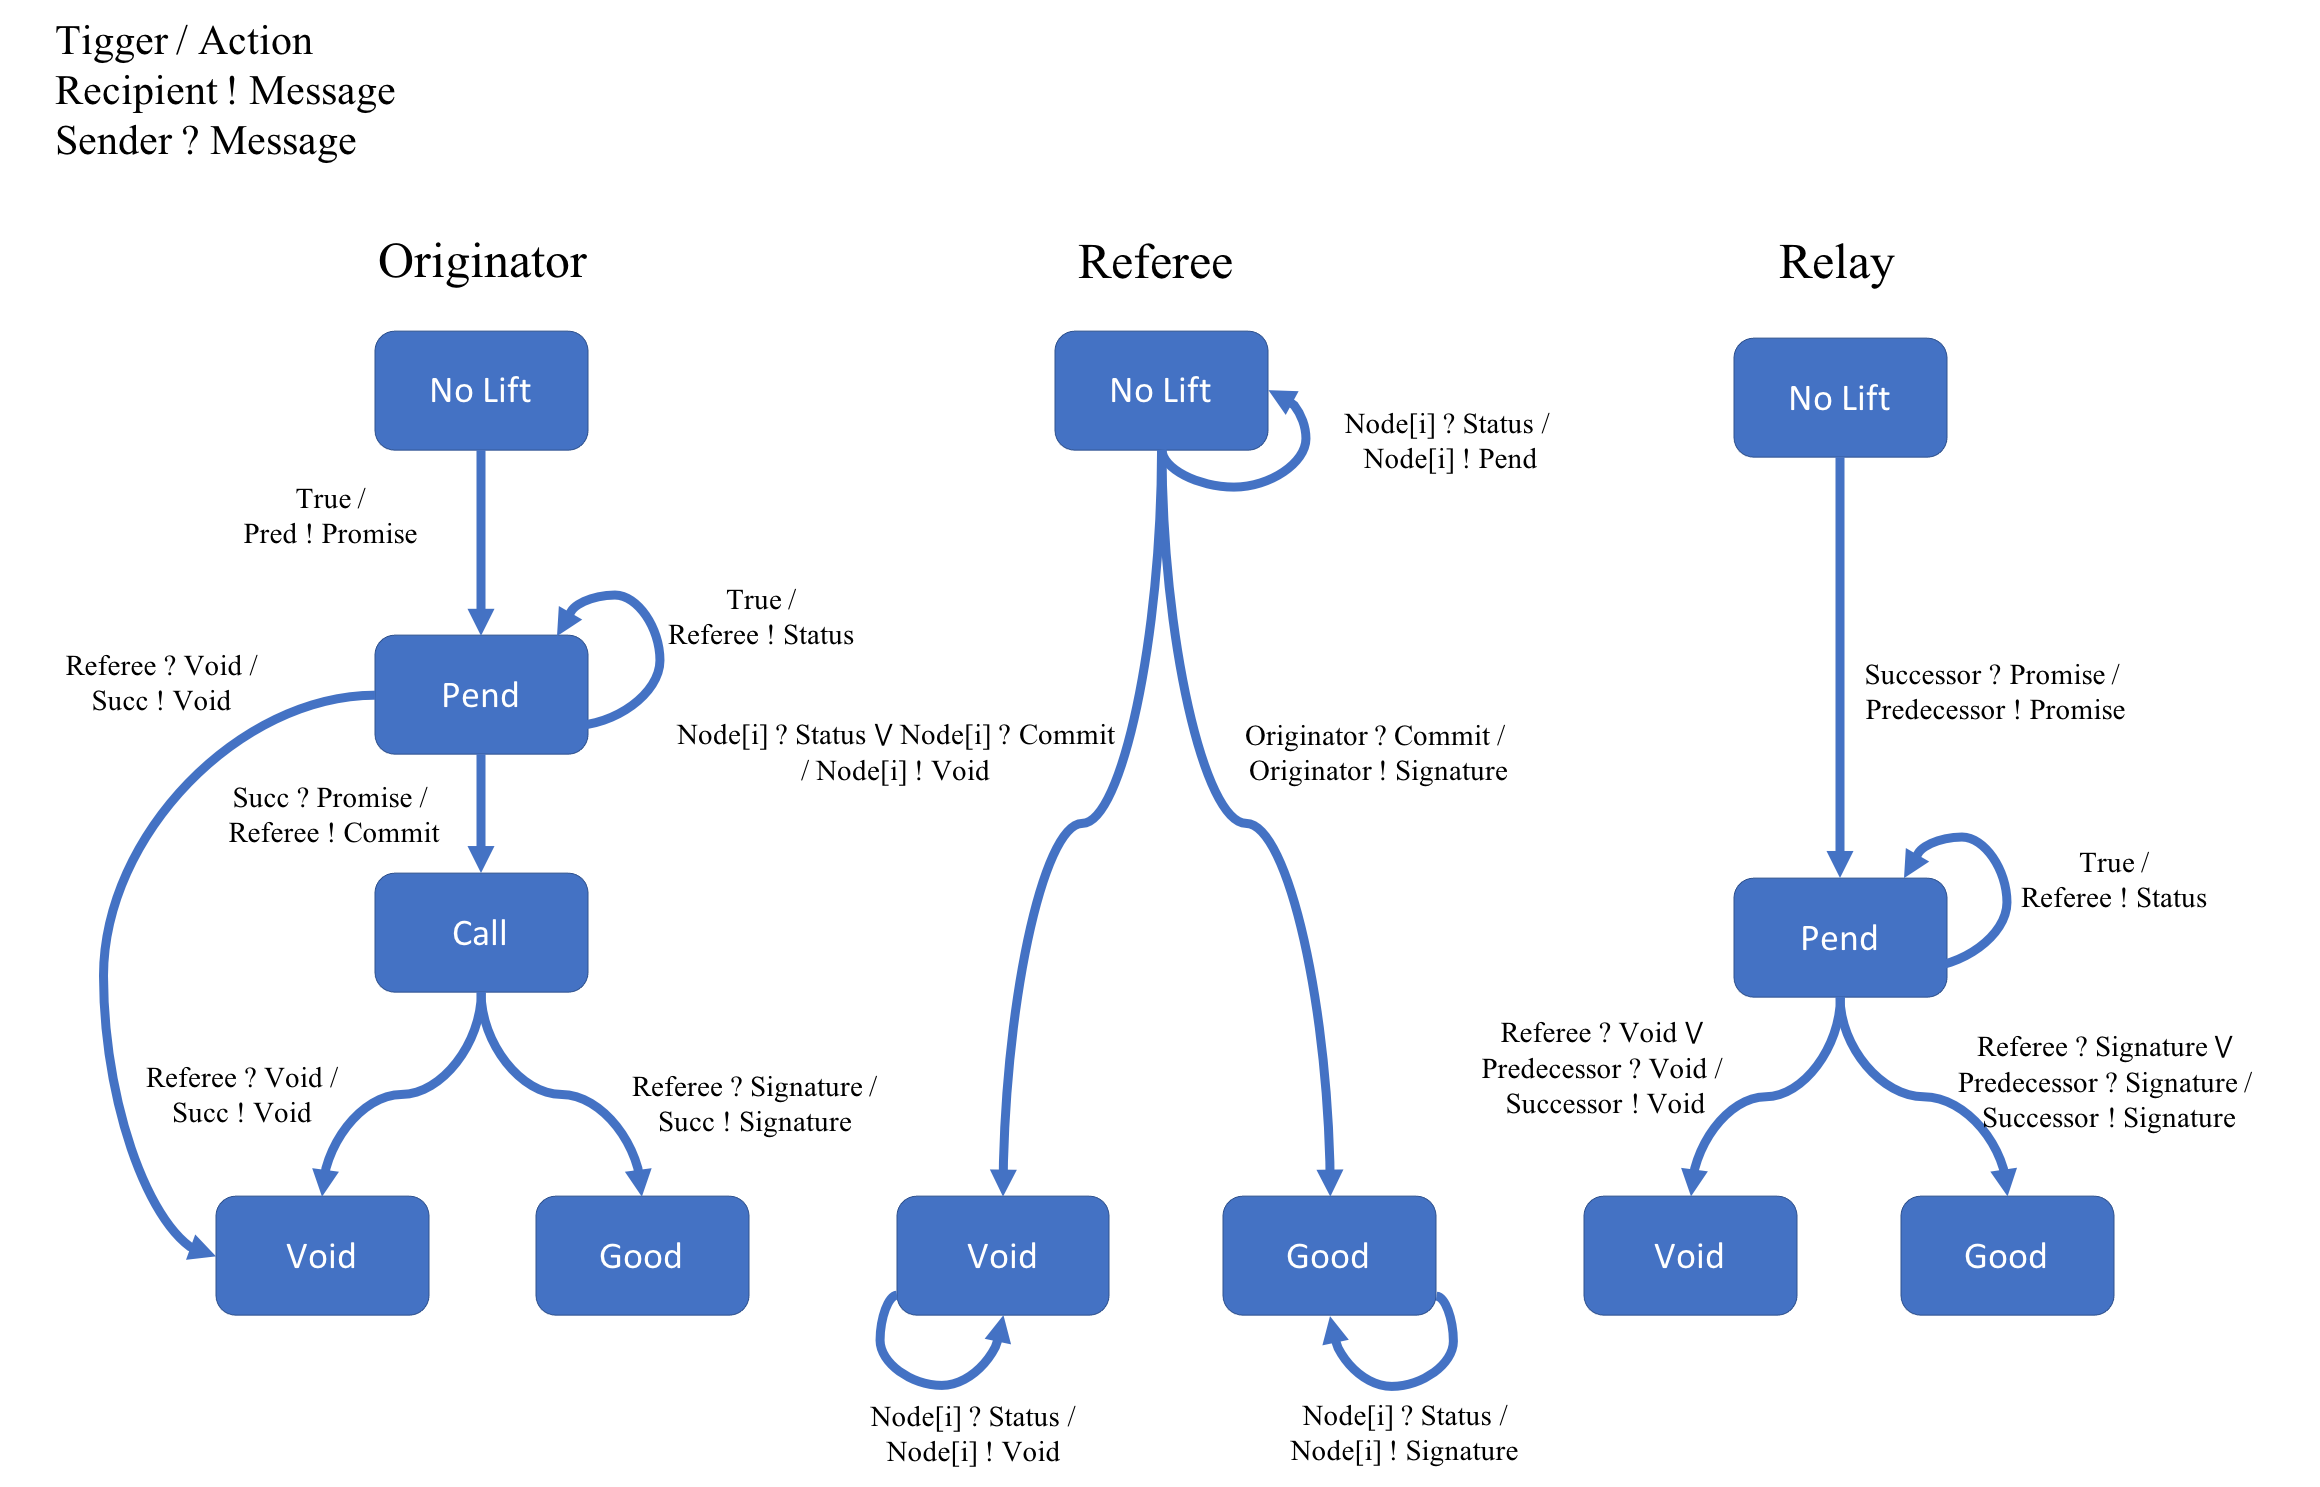
\includegraphics[scale=0.5]{LiftStatesSeperate.png}
    \caption{Lift States Diagram}
    \label{fig:liftStates}
\end{figure}

Fig. \ref{fig:liftStates} describes the behavior expected from each of these equivalence classes as mealy machines.
These mealy machines are based on the state machines Bateman provides to define the protocol. \cite{bateman_state_machines} 
In the figure, each box represents the state of the lift from the perspective of the node, and each arrow represents a change in state and an associated action that is taken during the transition from one state to the next. Each transition is labeled with a condition that must be true for the transition to be taken, separated by a $/$ from an action that is taken during the transition. Each node has stored within its state the network ID of its predecessor (Pred), its successor (Succ), and the Referee. A transition can be made conditional on receiving a particular message from a particular network ID. This case is written in the form \emph{sender} $?$ \emph{message\_type}. As an action during a transition, nodes may transmit a particular message to a particular network ID. This case is written in the form \emph{recipient} $!$ \emph{message\_type}. 

\section{Plan of Work}

The strategy for this analysis will be to split the problem into three sub-problems. The first sub-problem will consider a lift that has exactly 3 nodes--the originator, the referee, and one relay node--and ensure that all the properties hold for this small example. The next sub-problem will consider replacing the relay node with a chain of 2 or more relay nodes and prove that all the properties continue to hold, for the non-relay nodes. The final sub-problem will be to prove that the properties hold any chain of n relay nodes when the ends of the chain receive any messages supported by the protocol. 

The first sub-problem will be solved through model checking. The model will consist of three nodes: an originator, a referee, and one relay node. Each node will implement the respective state machine described above. We will admit in our model that messages can experience arbitrarily long delays, and may never be received. However, we add an exception that messages to and from the referee will eventually be received.  We assume that all participants will follow the protocol, but may become inactive and experience unbounded delays.  The referee, however, will always be active. We also assume that nodes only appear once in the circuit and that nodes only participate in one lift at a time.

We will solve the second sub-problem in the proof assistant Coq. We will define a partial order of events based on the state machines described above. This partial order will identify which events must occur sequentially as defined by the protocol. Using this partial order, we can define the set of event traces that can occur in a given system that is constrained by that partial order. 
We can then use the set of traces produced by the original 3 node system to form an \emph{expression context}. This set of traces is the same set of traces that the model checker explored exhaustively to prove that the properties hold in a simple 3 node system.
The model checking result will serve as the base case in an inductive proof. Next, we define a conformation relation. The conformation relation relates one set of traces to another. A set of traces $T$ conforms to $T'$ if $T'$ can be projected onto $T$ such that when you hide the states in the traces connected with entities that changed in the system the resulting traces are equivalent to the traces of the unchanged system. That is to say, we will prove:
$$\forall T, T \in TR(S) \longleftrightarrow T \in Proj(TR(S'), S)$$
Where $TR(S)$ defines the set of possible traces for a given system, and $Proj(TR(S'), S)$ projects the set of possible traces in system $S'$ onto system $S$ by hiding states of entities that are not in system $S$. 

Finally, for the third sub-problem we will expand the model in the first sub-problem to include 5 nodes. One originator, one referee, and 3 relay nodes. With this result we can prove that the interactions of 3 relay nodes in a chain conform to the required properties. Then we can use the conformance proven in the second sub-problem to expand those model checking results. By replacing the middle relay node with a chain of 2 or more relay nodes we can expand the chain to any number of nodes. 

Once all three sub-problems are solved, We can admit the model checking results from the first and third sub-problem as a base case, and use the lemmas proven in the second sub-problem to prove that a chain of $n$ relay nodes can always be safely replaced with a chain of $n+1$ relay nodes and the system's behavior will still conform to the required properties. This is an inductive step that allows us to construct a proof of correctness for a lift with any number of nodes. 

\section{Related Work}
 
 Nakamoto describes how transferable digital tokens can be double-spent. The paper introduces bitcoins and describes the proof of work method of overcoming this problem which is often referred to as blockchain technology. \cite{bitcoin} 

 Bateman recognizes that the double spending problem is present only in digital currencies that are both duplicatable and transferable. Blockchain technology prevents digital tokens from being duplicated. MyCHIPs instead is designed with non-transferable tokens. MyCHIPs utilizes credit lifts to allow these non-transferable tokens to be virtually fungible and to allow for effective transactions to be made. 
 
 Huang, Ogles, and Mercer prove that \emph{doesn't commute}, a weakened version of the happens-before relation, is sound for certain common classes of task parallel programs. They present a mechanized proof that proves properties for all traces constrained by a partial order. The methods demonstrated by Huang, Ogles, and Mercer can be utilized in this work's mechanized proof that the larger system conforms to the behavior of the smaller system. \cite{ben_DC}

 Bhargavan et. al. Verify Smart Contracts \cite{SmartContracts}. Smart contracts are a type of distributed computation where the program that is executed is secured in a blockchain. While not directly related, smart contracts have the same financial stakes MyCHIPs have and some of their techniques could give inspiration.  Bhargavan et. al, translated the smart contract code into a functional programming language, F*, aimed at verification. This allowed for contract verification based on F* type-checking.
 
 
 Fischer, Lynch, and Paterson,\cite{Fischer} prove the impossibility of consensus on even a Boolean, with even one faulty (or malicious) process. However, this is only true if the processes don't have synchronized clocks. This proof shows the necessity of the referee with strong reachability requirements for the lift algorithm to always eventually reach a consensus on if the lift should commit or be nullified.
 
 
 Schneider summarizes and frames many fault-tolerant distributed algorithms in the framework of  machines\cite{StateMachine}. He shows how many common algorithms are isomorphic to, and can be derived using, the state machine approach. It is a helpful method to characterize and compare different approaches.
 
 Lamport\cite{Lamport}, describes a refinement process that takes a distributed fault-tolerant consensus algorithm and hardens it to be tolerant of byzantine actors through a process he calls \emph{byzantizing.} This method may be useful in future work to ensure the MyCHIPs protocol follows key principles of Byzantine hard protocols.
 
 Delzanno, Tatarek, and Traverso, model check a common consensus algorithm called Paxos in Spin. Their spin constructs provide helpful examples of how distributed algorithms are efficiently modeled.\cite{Delzanno_2014}
 
 Konnov, Veith, and Widder explore the unsolved problems associated with model checking distributed algorithms. This can serve as a hazard map of difficult unsolved problems. It would be unfortunate if solving a known problem that is tangential to this work becomes a prerequisite to finishing. This also can serve to give context to this work and show how it progresses towards solving some of these problems.\cite{Konnov}

\bibliographystyle{unsrt}
\bibliography{proposal}

\end{document}
